\documentclass[12pt, a4paper]{article}


\usepackage[margin=1in]{geometry} % full-width

% AMS Packages
\usepackage{amsmath}
\usepackage{amsthm}
\usepackage{amssymb}

% Unicode
\usepackage[utf8]{inputenc}
\usepackage{hyperref}

% Natbib
\usepackage[sort&compress,numbers,square]{natbib}
\bibliographystyle{mplainnat}

% Theorem, Lemma, etc
\theoremstyle{plain}
\newtheorem{theorem}{Theorem}
\newtheorem{corollary}[theorem]{Corollary}
\newtheorem{lemma}[theorem]{Lemma}
\newtheorem{claim}{Claim}[theorem]
\newtheorem{axiom}[theorem]{Axiom}
\newtheorem{conjecture}[theorem]{Conjecture}
\newtheorem{fact}[theorem]{Fact}
\newtheorem{hypothesis}[theorem]{Hypothesis}
\newtheorem{assumption}[theorem]{Assumption}
\newtheorem{proposition}[theorem]{Proposition}
\newtheorem{criterion}[theorem]{Criterion}
\theoremstyle{definition}
\newtheorem{definition}[theorem]{Definition}
\newtheorem{example}[theorem]{Example}
\newtheorem{remark}[theorem]{Remark}
\newtheorem{problem}[theorem]{Problem}
\newtheorem{principle}[theorem]{Principle}

\usepackage{graphicx, color}
\graphicspath{{fig/}}

\usepackage{algorithm, algpseudocode} % use algorithm and algorithmicx for typesetting algorithms
\usepackage{mathrsfs} % for \mathscr command

\usepackage{parskip}

\usepackage{setspace}
\onehalfspacing % Adjust line spacing

% Author info
\title{
CS-E4660 - Advanced Topics in Software Systems
\large{Planning Document}
}
\author{Linus Jern}

\begin{document}
\maketitle

\subsection*{Problem Definition}

The problem for this project is the dynamic management of models and ML service provisioning with a focus on system latency given the accuracy constraints of any given request. 
This problem domain is quite complex, so some clarification is needed.
In this context, \textit{dynamic management of models and ML service provisioning} means the dynamic control of:
\begin{itemize}
    \item Model size
    \item Resource Utilization
\end{itemize}

An example of a system where this might be worth exploring is a system with strict latency requirements, but quite loose accuracy requirements.
In such a system, instead of letting each inference node sequentially handle the incoming queue of requests, the node might choose to preempt the queue and take the next job if the system resource utilization of it's own resources are low enough.
In addition to preempting the sequentiality, the node might choose a smaller, and thus faster with less resources, model if the circumstances allow.

What are the circumstances that would allow this compromise?
If the task is of a type that has a accuracy requirement or threshold which is low enough to compromise for a smaller and/or less accurate model, this preempting can occur.

See figure \autoref{plot_plot}, for a rough drawing of the idea space.
\begin{figure}[H]
    \centering
    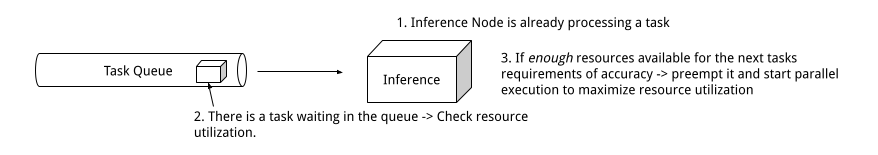
\includegraphics[width=\textwidth]{atss.png}
    \caption{Rough Drawing of the Situation}
    \label{plot_plot}
\end{figure}








    

\end{document}